\chapter{Marco Teórico}\label{cap:marco}
El marco teórico reúne los fundamentos matemáticos que sustentan el funcionamiento de una red neuronal artificial y los fundamentos técnicos del lenguaje Rust que justifican su elección. El capítulo avanza desde los objetos elementales ---vectores y matrices--- hasta el algoritmo completo de entrenamiento, y cada ecuación numerada tiene una implementación directa en el código fuente del proyecto, indicada en el texto para facilitar la trazabilidad entre la teoría y la práctica.

\section{Fundamentos de álgebra lineal}
El álgebra lineal proporciona el lenguaje con el que se describen los datos y las transformaciones de una red neuronal. Una entrada se representa como un vector, los parámetros de una capa como una matriz y un vector, y el procesamiento de la capa como una transformación afín seguida de una función no lineal \citep{strang2016,deisenroth2020}.

\subsection{Vectores y matrices}
Un vector $\mathbf{x}\in\mathbb{R}^{n}$ es una lista ordenada de $n$ números reales, interpretada en este trabajo como vector columna. Una matriz $\mathbf{W}\in\mathbb{R}^{m\times n}$ es un arreglo rectangular de $m$ filas y $n$ columnas \citep{strang2016}. En la implementación, las matrices se almacenan en un único arreglo contiguo en orden por filas (\emph{row-major}), de modo que el elemento $w_{ij}$ ocupa la posición $i\cdot n + j$ (con índices desde cero). La estructura \texttt{Vector} de \texttt{src/math/vector.rs} y la estructura \texttt{Matrix} de \texttt{src/math/matrix.rs} materializan estas definiciones.

\subsection{Operaciones fundamentales}
Sean $\mathbf{x},\mathbf{y}\in\mathbb{R}^{n}$, $\mathbf{A}\in\mathbb{R}^{m\times k}$ y $\mathbf{B}\in\mathbb{R}^{k\times n}$. Las operaciones implementadas, con su complejidad temporal, son:
\begin{align}
\mathbf{x}\cdot\mathbf{y} &= \sum_{i=1}^{n} x_i y_i, &&\text{(producto punto, } O(n)\text{)}\label{eq:dot}\\
(\mathbf{A}\mathbf{B})_{ij} &= \sum_{l=1}^{k} a_{il}\, b_{lj}, &&\text{(producto matricial, } O(mkn)\text{)}\label{eq:matmul}\\
(\mathbf{x}\odot\mathbf{y})_i &= x_i\, y_i, &&\text{(producto de Hadamard, } O(n)\text{)}\label{eq:hadamard}\\
(\mathbf{A}^{\top})_{ij} &= a_{ji}, &&\text{(transpuesta, } O(mk)\text{)}\label{eq:transpuesta}\\
(\mathbf{x}\,\mathbf{y}^{\top})_{ij} &= x_i\, y_j. &&\text{(producto exterior, } O(n^2)\text{)}\label{eq:outer}
\end{align}
Estas operaciones solo están definidas cuando las dimensiones son compatibles; por ejemplo, el producto $\mathbf{A}\mathbf{B}$ exige que el número de columnas de $\mathbf{A}$ coincida con el número de filas de $\mathbf{B}$. En el proyecto, toda violación de dimensiones produce un error explícito en lugar de un resultado incorrecto.

\subsection{Interpretación geométrica}
El producto punto mide la alineación entre dos vectores: $\mathbf{w}\cdot\mathbf{x} = \lVert\mathbf{w}\rVert\,\lVert\mathbf{x}\rVert\cos\theta$. En consecuencia, el conjunto de puntos que satisface $\mathbf{w}\cdot\mathbf{x} + b = 0$ es un hiperplano con vector normal $\mathbf{w}$, que divide el espacio de entradas en dos semiespacios. El producto matriz-vector $\mathbf{W}\mathbf{x}$ calcula simultáneamente $m$ productos punto, uno por fila, y por ello describe de forma compacta el trabajo de $m$ neuronas que reciben la misma entrada. El producto exterior $\mathbf{u}\mathbf{v}^{\top}$, en cambio, produce una matriz de rango uno y aparece de forma natural al calcular el gradiente de los pesos de una capa (Ecuación~\eqref{eq:gradW}). La operación $\mathbf{W}^{\top}\mathbf{v}$ se implementa sin construir explícitamente la transpuesta, recorriendo la matriz por columnas, lo que ahorra memoria en la retropropagación.

\section{La neurona artificial}
La neurona artificial, inspirada en el modelo de \citet{mcculloch1943} y en el perceptrón de \citet{rosenblatt1958}, recibe un vector de entradas $\mathbf{x}\in\mathbb{R}^{n}$, lo combina linealmente con un vector de pesos $\mathbf{w}\in\mathbb{R}^{n}$ y un sesgo $b\in\mathbb{R}$, y aplica una función de activación $f$:
\begin{equation}
z = \mathbf{w}\cdot\mathbf{x} + b = \sum_{i=1}^{n} w_i x_i + b, \qquad a = f(z).\label{eq:neurona}
\end{equation}
La suma ponderada $z$ define un hiperplano en el espacio de entradas. Por ello, una única neurona solo puede separar clases que sean linealmente separables, limitación que \citet{minsky1969} formalizaron con el ejemplo de la compuerta XOR. Para XOR, una neurona con salida $a = f(w_1x_1 + w_2x_2 + b)$ y umbral en $z=0$ necesitaría simultáneamente $b<0$ (para $(0,0)\mapsto 0$), $w_1+b>0$ y $w_2+b>0$ (para $(1,0)$ y $(0,1)\mapsto 1$) y $w_1+w_2+b<0$ (para $(1,1)\mapsto 0$). Sumando las dos desigualdades intermedias se obtiene $w_1+w_2+2b>0$, es decir, $w_1+w_2+b>-b>0$, lo que contradice la última condición. La contradicción demuestra que ningún conjunto de parámetros resuelve el problema con una sola neurona, resultado que se observa experimentalmente en la Sección~\ref{sec:exp2}.

\section{Funciones de activación}
Las funciones de activación introducen no linealidad; sin ellas, la composición de varias capas seguiría siendo una transformación lineal, pues $\mathbf{W}_2(\mathbf{W}_1\mathbf{x}+\mathbf{b}_1)+\mathbf{b}_2 = (\mathbf{W}_2\mathbf{W}_1)\mathbf{x} + (\mathbf{W}_2\mathbf{b}_1+\mathbf{b}_2)$ \citep{goodfellow2016}. La Figura~\ref{fig:activaciones} muestra las dos funciones no lineales implementadas y sus derivadas.

\begin{figure}[!htbp]
\caption{Funciones de activación Sigmoid y ReLU con sus derivadas}\label{fig:activaciones}
\centering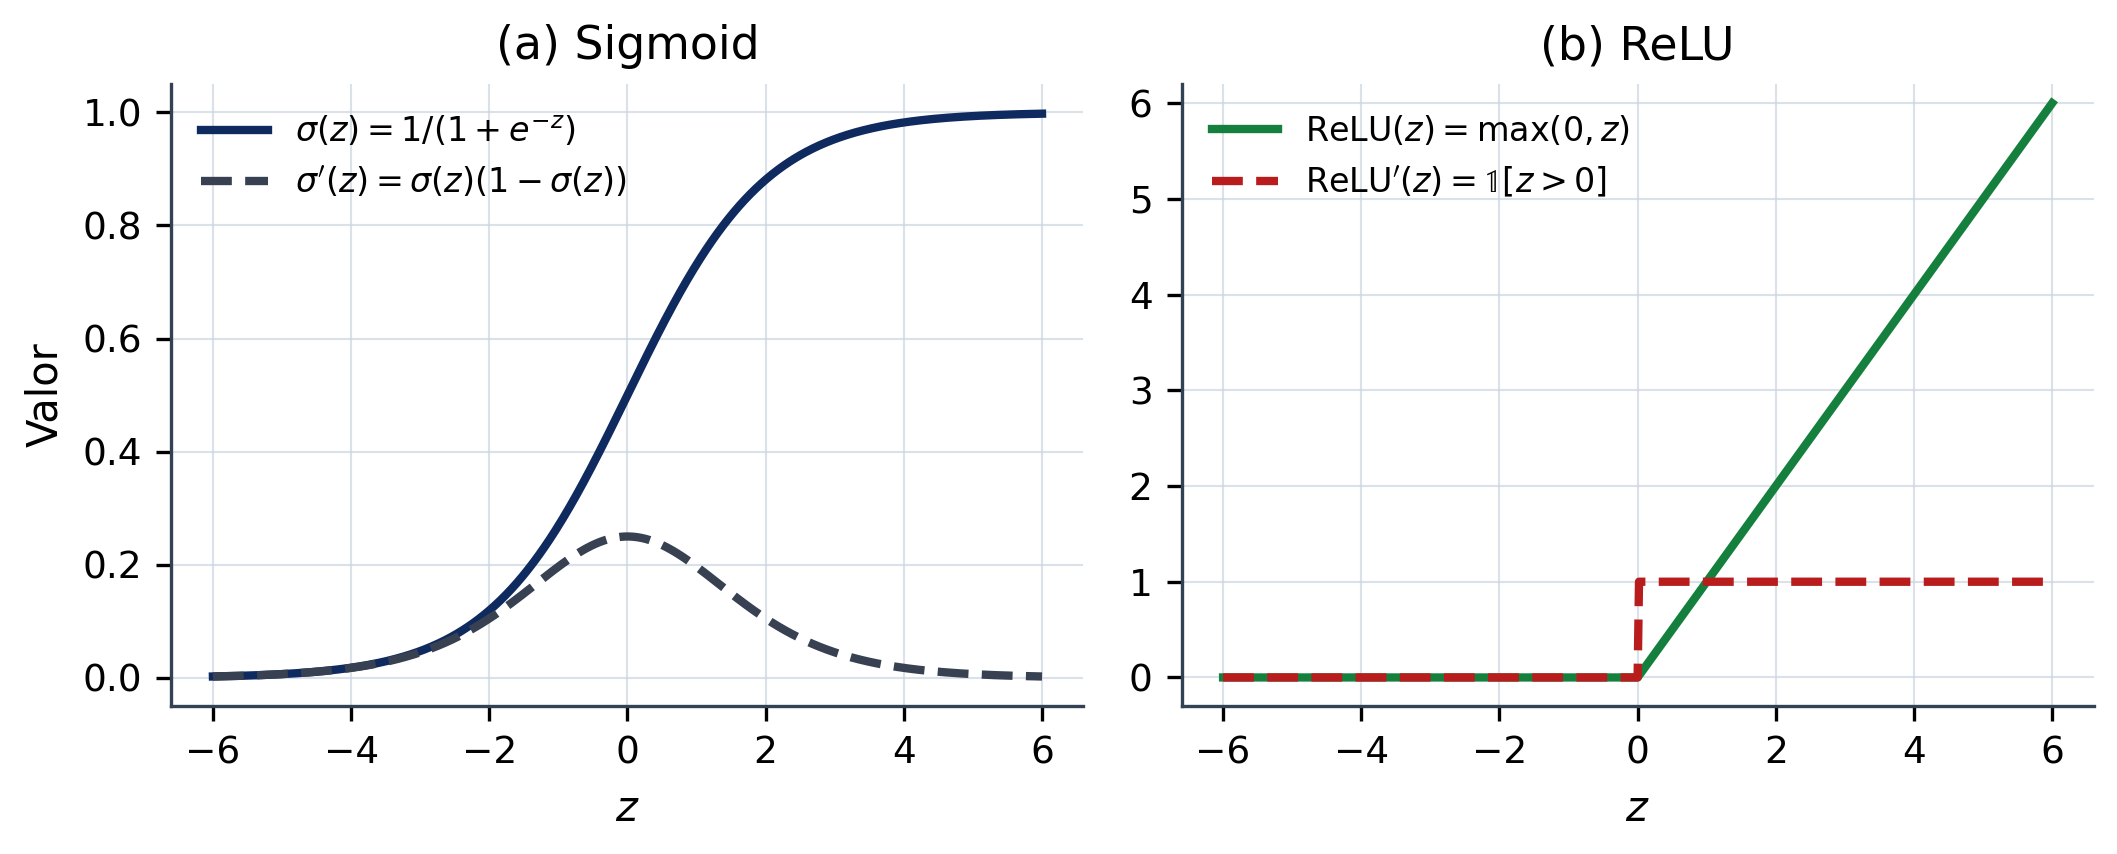
\includegraphics[width=\textwidth]{figuras/fig01_activaciones.png}
\fuente{(a) Sigmoid y su derivada, con máximo $0.25$ en $z=0$. (b) ReLU y su derivada escalón. Curvas trazadas con las Ecuaciones~\eqref{eq:sigmoid} y~\eqref{eq:relu}, idénticas a las implementadas en \texttt{src/nn/activation.rs}.}
\end{figure}

\subsection{Función Sigmoid}
La función logística o Sigmoid transforma cualquier número real en un valor del intervalo $(0,1)$, por lo que su salida puede interpretarse como una probabilidad o un grado de activación:
\begin{equation}
\sigma(z) = \frac{1}{1+e^{-z}}, \qquad \sigma'(z) = \sigma(z)\,\bigl(1-\sigma(z)\bigr).\label{eq:sigmoid}
\end{equation}
La derivada se obtiene aplicando la regla del cociente:
\begin{equation*}
\sigma'(z) = \frac{e^{-z}}{(1+e^{-z})^2} = \frac{1}{1+e^{-z}}\cdot\frac{e^{-z}}{1+e^{-z}} = \frac{1}{1+e^{-z}}\cdot\Bigl(1-\frac{1}{1+e^{-z}}\Bigr) = \sigma(z)\bigl(1-\sigma(z)\bigr).
\end{equation*}
Su valor máximo es $0.25$ en $z=0$, y tiende a cero cuando $|z|$ crece. Esta saturación explica la lentitud del aprendizaje cuando las neuronas reciben entradas de gran magnitud y, en redes profundas, el desvanecimiento del gradiente, pues el producto de muchas derivadas menores o iguales a $0.25$ decrece exponencialmente con la profundidad \citep{lecun1998}. Para evitar desbordamientos numéricos al evaluar $e^{-z}$ con $z$ muy negativo, la implementación usa la forma equivalente $\sigma(z) = e^{z}/(1+e^{z})$ cuando $z<0$.

\subsection{Función ReLU}
La unidad lineal rectificada (ReLU) anula los valores negativos y conserva los positivos:
\begin{equation}
\mathrm{ReLU}(z) = \max(0, z), \qquad \mathrm{ReLU}'(z) = \begin{cases}1 & z>0\\ 0 & z\le 0\end{cases}\label{eq:relu}
\end{equation}
ReLU es computacionalmente económica, no se satura para entradas positivas y mitiga el desvanecimiento del gradiente en redes profundas \citep{glorot2010,he2015}. En $z=0$ la derivada no existe; por convención se adopta el valor $0$. Su principal inconveniente es que una neurona cuya entrada permanece negativa deja de aprender, fenómeno conocido como neurona muerta.

\subsection{Función lineal}
Para problemas de regresión se utiliza la identidad $f(z)=z$, cuya derivada es $f'(z)=1$. Una red con una única neurona lineal y pérdida MSE equivale a una regresión lineal por mínimos cuadrados resuelta iterativamente, lo que hace del Experimento~1 un caso de prueba con solución analítica conocida.

\section{Función de pérdida: error cuadrático medio}
La función de pérdida cuantifica la discrepancia entre la predicción de la red y el valor esperado, y es la magnitud que el entrenamiento minimiza. Dado un vector de predicciones $\hat{\mathbf{y}}\in\mathbb{R}^{n}$ y un vector objetivo $\mathbf{y}\in\mathbb{R}^{n}$, el error cuadrático medio y su gradiente son:
\begin{equation}
\mathcal{L}(\hat{\mathbf{y}},\mathbf{y}) = \frac{1}{n}\sum_{i=1}^{n}(\hat{y}_i - y_i)^2, \qquad \frac{\partial\mathcal{L}}{\partial \hat{y}_i} = \frac{2}{n}(\hat{y}_i - y_i).\label{eq:mse}
\end{equation}
El MSE es siempre no negativo, vale cero únicamente cuando la predicción coincide exactamente con el objetivo y penaliza con mayor peso los errores grandes debido al término cuadrático \citep{bishop2006}. Desde la perspectiva estadística, minimizar el MSE equivale a maximizar la verosimilitud bajo la hipótesis de ruido gaussiano. En el Experimento~2, un MSE de $0.25$ corresponde a predecir $0.5$ para todas las entradas de XOR, valor de referencia útil para interpretar el estancamiento del perceptrón.

\section{Red neuronal multicapa}
Una red multicapa (\emph{multilayer perceptron}) organiza las neuronas en $L$ capas densas, en las que cada neurona de una capa recibe todas las salidas de la capa anterior. Para la capa $l$ con $n_{l-1}$ entradas y $n_l$ neuronas, los parámetros son la matriz $\mathbf{W}^{(l)}\in\mathbb{R}^{n_l\times n_{l-1}}$ y el vector $\mathbf{b}^{(l)}\in\mathbb{R}^{n_l}$, de modo que la capa tiene $n_l(n_{l-1}+1)$ parámetros. La propagación hacia adelante es:
\begin{equation}
\mathbf{z}^{(l)} = \mathbf{W}^{(l)}\mathbf{a}^{(l-1)} + \mathbf{b}^{(l)}, \qquad \mathbf{a}^{(l)} = f^{(l)}\bigl(\mathbf{z}^{(l)}\bigr), \qquad \mathbf{a}^{(0)} = \mathbf{x}.\label{eq:forward}
\end{equation}
Aplicando esta fórmula, la red 2-4-1 del Experimento~2 tiene $4\cdot(2+1) + 1\cdot(4+1) = 17$ parámetros, y la red 25-10-5 del Experimento~3 tiene $10\cdot 26 + 5\cdot 11 = 315$. El teorema de aproximación universal garantiza que una red con una sola capa oculta y un número suficiente de neuronas con activación sigmoidal puede aproximar cualquier función continua en un dominio compacto con precisión arbitraria \citep{cybenko1989,hornik1989}. El teorema asegura la existencia de los parámetros, pero no indica cómo encontrarlos; esa tarea corresponde al algoritmo de entrenamiento.

\section{Retropropagación del error}
La retropropagación (\emph{backpropagation}) calcula eficientemente el gradiente de la pérdida respecto a todos los parámetros aplicando la regla de la cadena desde la salida hacia la entrada \citep{rumelhart1986}. Se define el error local de la capa $l$ como $\boldsymbol{\delta}^{(l)} = \partial\mathcal{L}/\partial\mathbf{z}^{(l)}$, es decir, la sensibilidad de la pérdida respecto a la suma ponderada de cada neurona.

\subsection{Regla de la cadena}
Si $\mathcal{L}$ depende de $z$ a través de una cadena de funciones $z\mapsto a\mapsto \mathcal{L}$, la regla de la cadena establece que $\frac{d\mathcal{L}}{dz} = \frac{d\mathcal{L}}{da}\cdot\frac{da}{dz}$. Cuando una variable influye en la pérdida a través de varios caminos, las contribuciones se suman: $\frac{\partial\mathcal{L}}{\partial a_j} = \sum_k \frac{\partial\mathcal{L}}{\partial z_k}\frac{\partial z_k}{\partial a_j}$. Estas dos reglas son suficientes para derivar todo el algoritmo.

\subsection{Derivación paso a paso}
Para la capa de salida $L$, por la regla de la cadena:
\begin{equation}
\delta_j^{(L)} = \frac{\partial\mathcal{L}}{\partial a_j^{(L)}}\cdot\frac{\partial a_j^{(L)}}{\partial z_j^{(L)}} = \frac{2}{n_L}\bigl(a_j^{(L)}-y_j\bigr)\, f'\bigl(z_j^{(L)}\bigr)
\;\Longrightarrow\; \boldsymbol{\delta}^{(L)} = \nabla_{\mathbf{a}}\mathcal{L}\odot f'\bigl(\mathbf{z}^{(L)}\bigr).\label{eq:deltaL}
\end{equation}
Para una capa oculta $l$, cada $z_j^{(l)}$ influye en la pérdida a través de todas las neuronas $k$ de la capa siguiente:
\begin{equation}
\begin{split}
\delta_j^{(l)} &= \sum_{k}\frac{\partial\mathcal{L}}{\partial z_k^{(l+1)}}\frac{\partial z_k^{(l+1)}}{\partial a_j^{(l)}}\frac{\partial a_j^{(l)}}{\partial z_j^{(l)}} = \Bigl(\sum_k w_{kj}^{(l+1)}\delta_k^{(l+1)}\Bigr) f'\bigl(z_j^{(l)}\bigr)\\
\Longrightarrow\quad \boldsymbol{\delta}^{(l)} &= \bigl(\mathbf{W}^{(l+1)\top}\boldsymbol{\delta}^{(l+1)}\bigr)\odot f'\bigl(\mathbf{z}^{(l)}\bigr).
\end{split}\label{eq:deltal}
\end{equation}
Como $z_j^{(l)} = \sum_i w_{ji}^{(l)}a_i^{(l-1)} + b_j^{(l)}$, se cumple $\partial z_j^{(l)}/\partial w_{ji}^{(l)} = a_i^{(l-1)}$ y $\partial z_j^{(l)}/\partial b_j^{(l)} = 1$, de modo que los gradientes de los parámetros resultan:
\begin{equation}
\frac{\partial\mathcal{L}}{\partial\mathbf{W}^{(l)}} = \boldsymbol{\delta}^{(l)}\,\mathbf{a}^{(l-1)\top}, \qquad \frac{\partial\mathcal{L}}{\partial\mathbf{b}^{(l)}} = \boldsymbol{\delta}^{(l)}.\label{eq:gradW}
\end{equation}
El costo de la retropropagación es del mismo orden que el de la propagación hacia adelante, $O(P)$, donde $P$ es el número total de parámetros, lo que la hace mucho más eficiente que estimar cada derivada por separado, cuyo costo sería $O(P^2)$ \citep{baydin2018}. En la implementación, cada capa guarda en caché su entrada $\mathbf{a}^{(l-1)}$ y su suma ponderada $\mathbf{z}^{(l)}$ durante la propagación hacia adelante, y el método \texttt{Layer::backward} aplica literalmente las Ecuaciones~\eqref{eq:deltal} y~\eqref{eq:gradW}.

\section{Descenso de gradiente}
El descenso de gradiente actualiza cada parámetro en dirección opuesta al gradiente, que es la dirección de máximo crecimiento local de la pérdida, con una tasa de aprendizaje $\alpha>0$:
\begin{equation}
\mathbf{W}^{(l)} \leftarrow \mathbf{W}^{(l)} - \alpha\,\frac{\partial\mathcal{L}}{\partial\mathbf{W}^{(l)}}, \qquad \mathbf{b}^{(l)} \leftarrow \mathbf{b}^{(l)} - \alpha\,\frac{\partial\mathcal{L}}{\partial\mathbf{b}^{(l)}}.\label{eq:gd}
\end{equation}
La justificación proviene de la aproximación de Taylor de primer orden: para un desplazamiento pequeño $\Delta\boldsymbol{\theta} = -\alpha\nabla\mathcal{L}$, se tiene $\mathcal{L}(\boldsymbol{\theta}+\Delta\boldsymbol{\theta}) \approx \mathcal{L}(\boldsymbol{\theta}) - \alpha\lVert\nabla\mathcal{L}\rVert^2 \le \mathcal{L}(\boldsymbol{\theta})$. En la variante estocástica (SGD) utilizada en este proyecto, la actualización se realiza después de cada muestra, lo que introduce ruido en la trayectoria pero permite avanzar sin recorrer todo el conjunto de datos \citep{bottou2010}. Una tasa $\alpha$ muy pequeña produce un aprendizaje extremadamente lento; una tasa excesiva provoca oscilaciones, divergencia o saturación de las neuronas \citep{ruder2016}. Este comportamiento se verifica experimentalmente en la Sección~\ref{sec:exp2}.

\section{Inicialización de pesos}
Si todos los pesos se inicializan con el mismo valor, las neuronas de una capa reciben gradientes idénticos y nunca se diferencian, problema conocido como simetría. Si se inicializan con valores demasiado grandes, las neuronas Sigmoid se saturan desde el inicio; si son demasiado pequeños, la señal se atenúa al atravesar las capas. Por ello se emplea inicialización aleatoria uniforme en $[-\ell,\ell]$ con la regla de \citet{glorot2010} para Sigmoid y lineal, y la de \citet{he2015} para ReLU:
\begin{equation}
\ell_{\text{Xavier}} = \sqrt{\frac{6}{n_{\text{in}}+n_{\text{out}}}}, \qquad \ell_{\text{He}} = \sqrt{\frac{6}{n_{\text{in}}}}.\label{eq:init}
\end{equation}
Ambas reglas buscan que la varianza de las activaciones y de los gradientes se mantenga aproximadamente constante entre capas. Los sesgos se inicializan en cero, pues la asimetría ya la aportan los pesos.

\section{Verificación numérica de gradientes}
Una implementación incorrecta de la retropropagación puede producir una red que aprende parcialmente y ocultar el error. Para comprobar que las derivadas analíticas están correctamente implementadas, se compara cada componente del gradiente con su aproximación por diferencias centrales \citep{lecun1998,goodfellow2016}:
\begin{equation}
\frac{\partial\mathcal{L}}{\partial\theta} \approx \frac{\mathcal{L}(\theta+\varepsilon)-\mathcal{L}(\theta-\varepsilon)}{2\varepsilon}, \qquad \text{error relativo} = \frac{|g_{\text{num}}-g_{\text{ana}}|}{\max(|g_{\text{num}}|+|g_{\text{ana}}|,\,10^{-12})}.\label{eq:gradcheck}
\end{equation}
Desarrollando $\mathcal{L}(\theta\pm\varepsilon)$ en serie de Taylor, los términos de orden par se cancelan y el error de truncamiento resulta $O(\varepsilon^{2})$, frente a $O(\varepsilon)$ de la diferencia hacia adelante. Por ello, un error relativo muy pequeño indica que la retropropagación es correcta. El proyecto aplica esta verificación a todos los parámetros de redes 2-4-1, 3-5-4-2 y 25-10-5.

\section{Métricas de evaluación}
Para regresión se utiliza el propio MSE. Para clasificación se utiliza la exactitud (\emph{accuracy}), definida como la proporción de muestras correctamente clasificadas, y la matriz de confusión $\mathbf{C}\in\mathbb{N}^{K\times K}$, cuyo elemento $c_{ij}$ cuenta las muestras de clase real $i$ predichas como clase $j$:
\begin{equation}
\text{exactitud} = \frac{\sum_{i=1}^{K} c_{ii}}{\sum_{i=1}^{K}\sum_{j=1}^{K} c_{ij}}.\label{eq:accuracy}
\end{equation}
En clasificación binaria (XOR) se asigna la clase 1 cuando la salida es mayor o igual que $0.5$. En clasificación multiclase con codificación \emph{one-hot}, la clase predicha es $\hat{k} = \arg\max_k \hat{y}_k$ \citep{bishop2006}. La matriz de confusión complementa la exactitud porque revela qué clases se confunden entre sí, información que la exactitud global oculta.

\section{Fundamentos técnicos de Rust}
Rust es un lenguaje de programación de sistemas compilado, con tipado estático y fuerte, diseñado para ofrecer seguridad de memoria sin recolector de basura \citep{klabnik2023,matsakis2014}. Las siguientes subsecciones describen las características del lenguaje que intervienen directamente en el diseño del motor.

\subsection{Propiedad, préstamos y tiempos de vida}
El modelo de propiedad (\emph{ownership}) establece que cada valor tiene un único dueño y se libera automáticamente cuando su dueño sale de ámbito. Los préstamos (\emph{borrowing}) permiten referencias inmutables múltiples (\texttt{\&T}) o una única referencia mutable (\texttt{\&mut T}), lo que elimina en tiempo de compilación las carreras de datos y los accesos a memoria liberada \citep{blandy2021}. \citet{jung2018} demostraron formalmente la solidez de estas garantías en el proyecto RustBelt. La Figura~\ref{fig:memoria} muestra cómo se aplican estas reglas en el motor: la red posee sus capas, cada capa posee sus matrices y vectores en el montón, y las funciones de cálculo reciben referencias prestadas.

\begin{figure}[!htbp]
\caption{Modelo de memoria, propiedad y préstamos en el motor}\label{fig:memoria}
\centering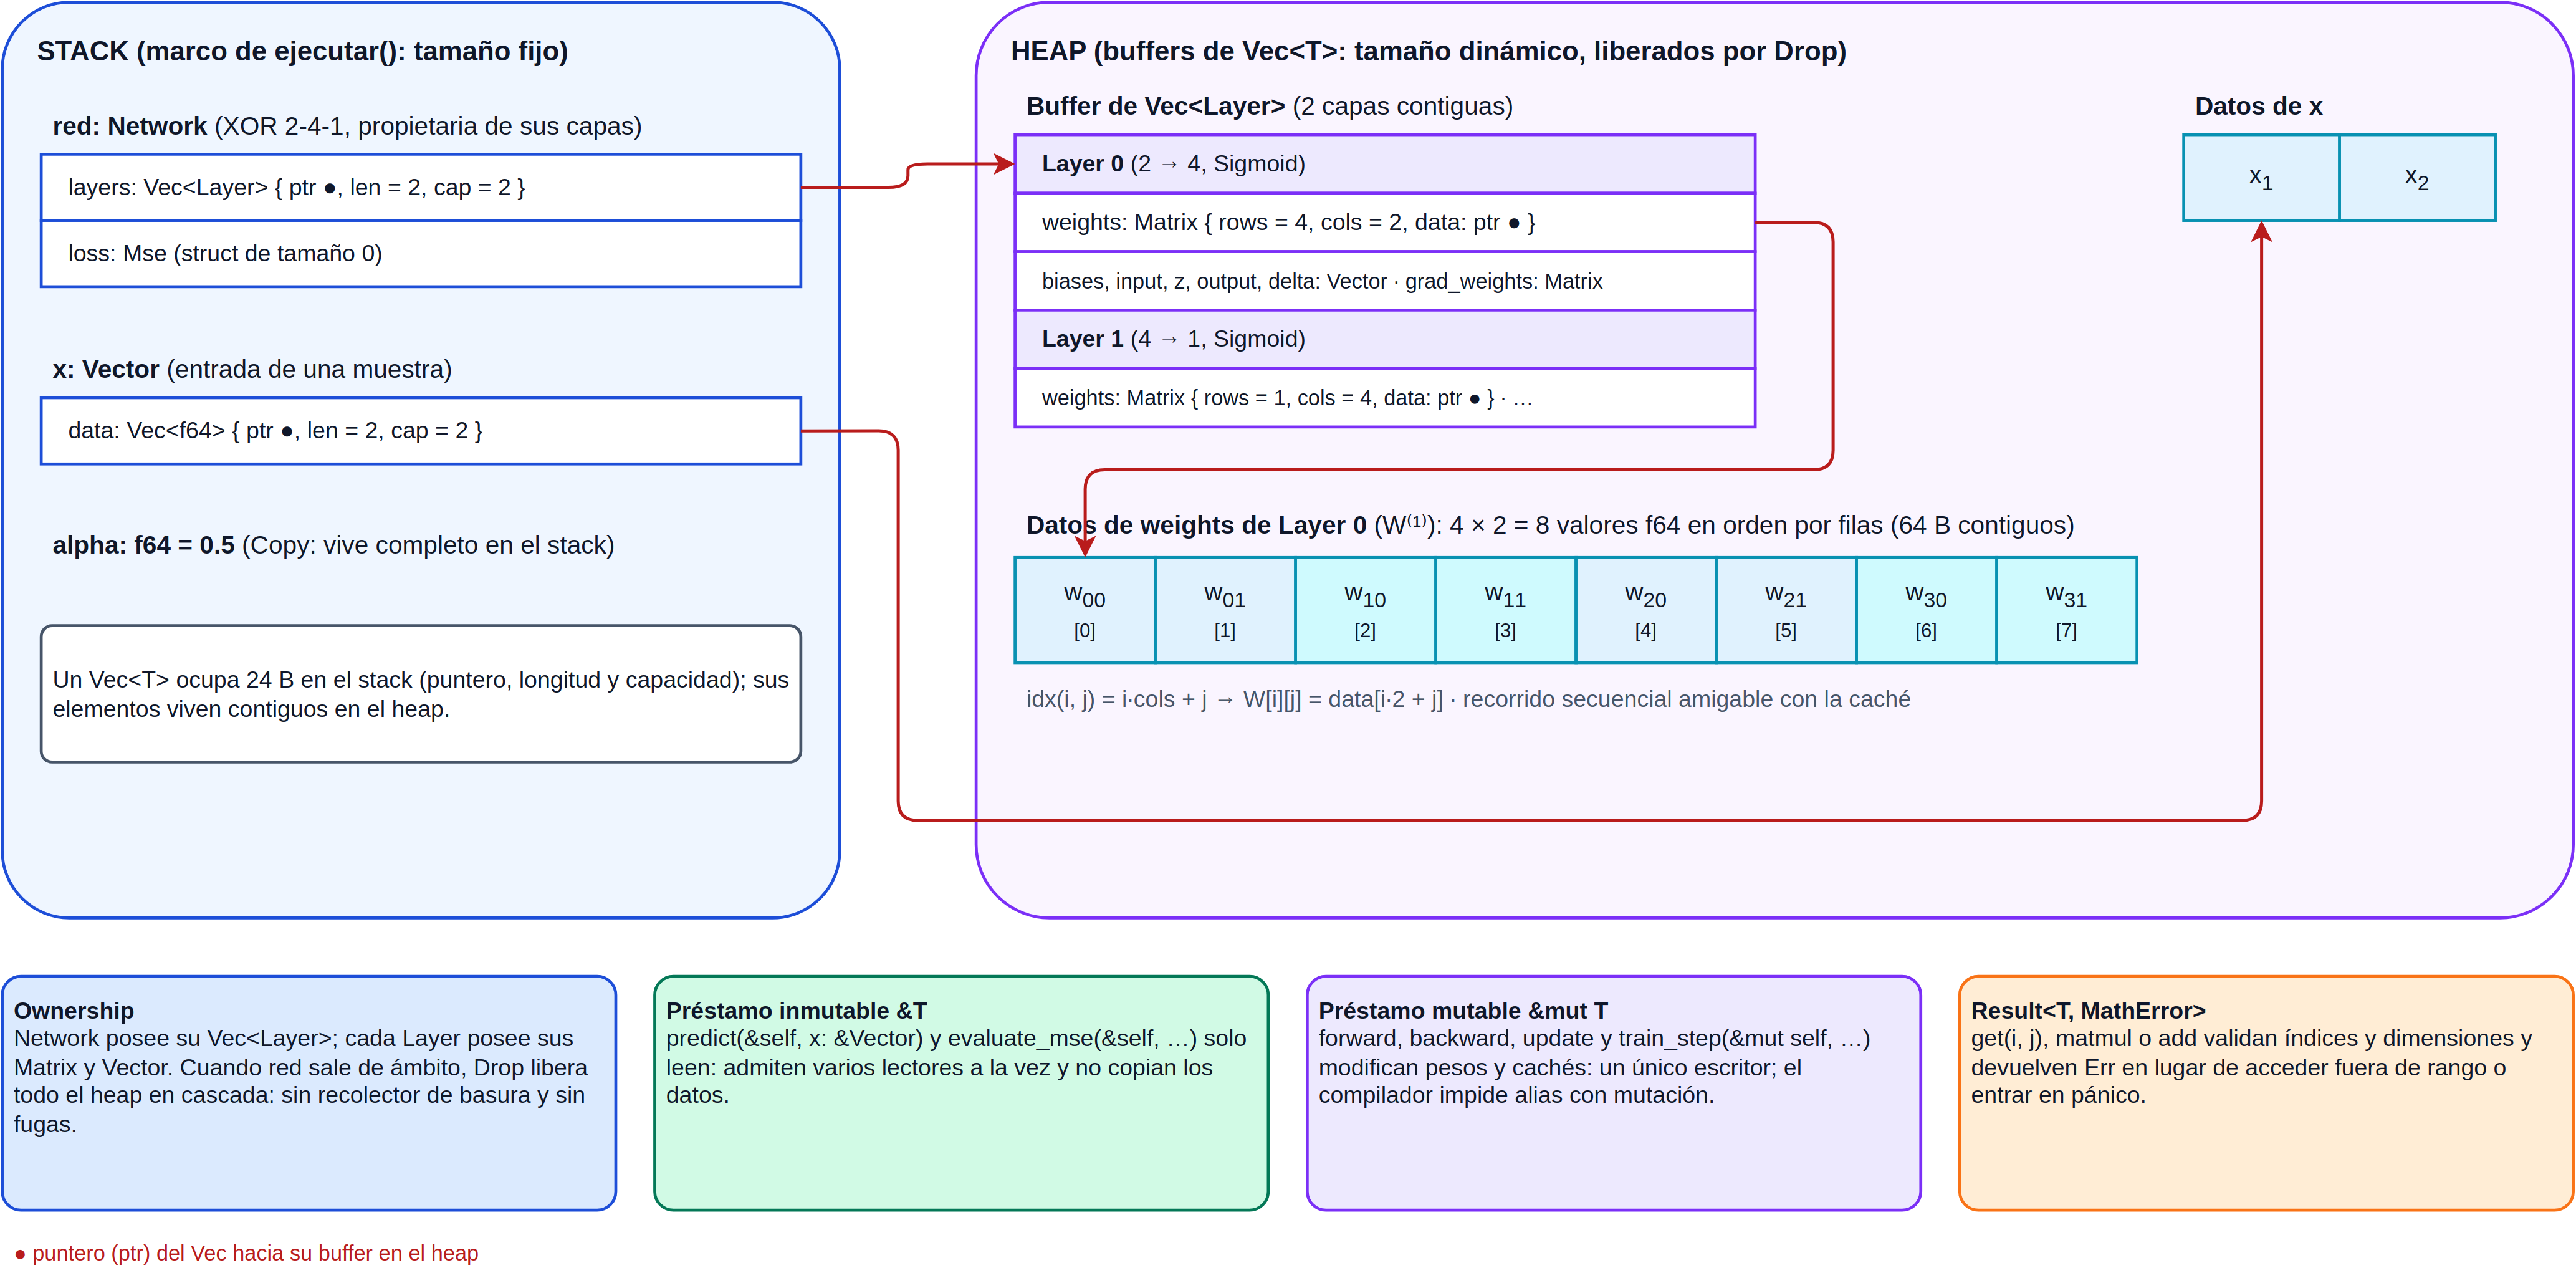
\includegraphics[width=\textwidth,height=0.55\textheight,keepaspectratio]{figuras/diag04_memoria_rust.png}
\fuente{La pila contiene las estructuras de control y el montón los arreglos de datos de cada capa. Diagrama editable: \texttt{diagramas/04\_memoria\_ownership\_rust.drawio}.}
\end{figure}

\subsection{Manejo explícito de errores}
Rust no utiliza excepciones. Las operaciones que pueden fallar devuelven \texttt{Result<T, E>}, que obliga al programador a tratar el error explícitamente. El operador \texttt{?} propaga el error al llamador de forma concisa. En este proyecto, toda operación de álgebra lineal devuelve \texttt{Result} con un tipo \texttt{MathError} que describe la operación y las dimensiones incompatibles, y los experimentos convierten esos errores, junto con los de entrada/salida, en un tipo \texttt{ExperimentError} mediante el trait \texttt{From}.

\subsection{Traits y abstracciones de costo cero}
Los \emph{traits} definen comportamiento compartido, de forma similar a las interfaces de otros lenguajes. El proyecto define los traits \texttt{ActivationFn} y \texttt{LossFn}, lo que permite añadir nuevas funciones sin modificar la red. Gracias a la monomorfización, el compilador genera código especializado para cada tipo concreto, de modo que estas abstracciones no tienen costo en tiempo de ejecución.

\subsection{Cargo, pruebas integradas y perfiles de compilación}
Cargo es el gestor de paquetes y sistema de compilación de Rust. Permite compilar en modo depuración o en modo optimizado (\texttt{--release}), ejecutar pruebas unitarias con \texttt{cargo test}, analizar el código con \texttt{cargo clippy} y generar documentación a partir de los comentarios \texttt{///} \citep{klabnik2023}. El perfil \emph{release} aplica optimizaciones del compilador LLVM, como la vectorización y la eliminación de comprobaciones redundantes, que reducen sustancialmente el tiempo de entrenamiento respecto al perfil de depuración.
